\begin{question}[topic=gsm,type=exam,tags={20150513}]
Eine kompensierte \underline{Reihenschluss}-Gleichstrommaschine hat folgende Daten. \\
Eine Leerlaufkennlinie $\frac{U_i}{I_E}$ bei $n=800 ~\frac{U}{min}$ ist gegeben (siehe Abb.\ref{fig:20150513}).\\
\begin{tabular}{L{2cm}l}
$I_{A,N}$ \dotfill &$280~A$\\
$U_{A,N}$ \dotfill & $300~V$ \\
$n_N$ \dotfill & $1200~\frac{U}{min}$
\end{tabular}
\begin{enumerate}
\item Wie groß ist die Spannungskonstante $k_1 \phi_N$ im Nennpunkt, das Nennmoment $M_N$ und die Nennleistung $P_N$ der Gleichstrommaschine? (\addpoints{2})
\item Berechnen Sie den Innenwiderstand $R_i$ (= Ankerwiderstand $R_A$ + Erregerwiderstand $R_E$) und den Wirkungsgrad $\eta_N$ im Nennpunkt. (\addpoints{2})
\item Bestimmen Sie die Drehzahl $n$ und das Drehmoment $M$ für eine Ankerspannung $U_A = 200~V$ und $I_A=140~A$. (\addpoints{1})
\item Skizzieren Sie die Drehzahl-Drehmoment Kennlinie ($M/n$) bei Nennspannung $U_{A,N} = 300~V$ im Bereich ca. $0,2 M_N$ bis $M_N$. (\addpoints{2})
\item Die Maschine wird bei $n=500~ U/min$ auf einen Widerstand $R_L$ gebremst. Dimensionieren Sie den Bremswiderstand $R_L$ so, dass ein anfänglicher Bremsstrom von $200~A$ fließt und geben Sie die Ankerspannung $U_A$ an den Maschinenklemmen und das Bremsmoment zu Begin der Bremsung an. (\addpoints{3})
\end{enumerate}
\begin{figure}[H] 
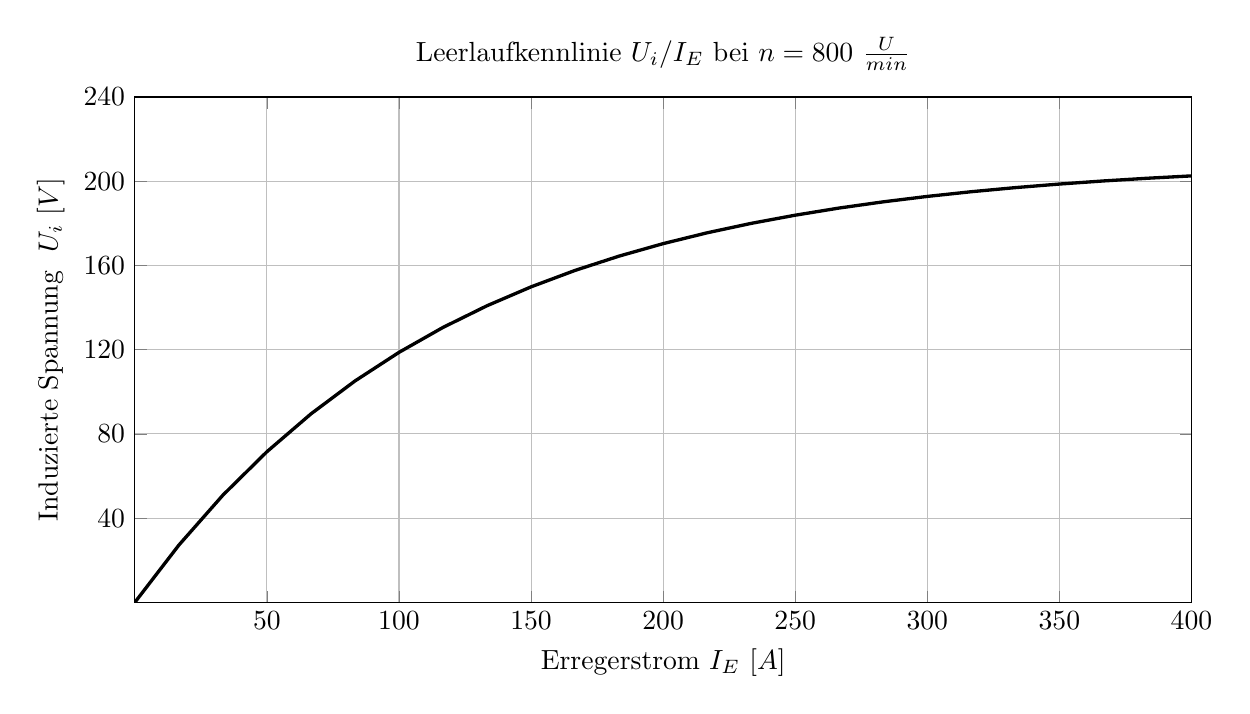
\begin{tikzpicture}
\begin{axis}[title={{Leerlaufkennlinie} $U_i/I_E$ {bei} $n=800 ~\frac{U}{min}$},xlabel={{Erregerstrom }$I_E \, \left[A\right]$ }, ylabel={{Induzierte Spannung } $U_i \, \left [V\right]$},
xtick= {50,100,150,200,250,300,350,400},
xmin = 0,xmax = 400,width=15cm, height= 8cm,
ytick= {40,80,120,160,200,240},
ymin = 0 , ymax = 240,grid=major]
\addplot+
[id=exp,color=black,mark=none,domain=0:400, very thick]{210*(1-exp(-x/120))};
\end{axis}
\end{tikzpicture}
\caption{Leerlaufkennlinie} \label{fig:20150513}
\end{figure}
\end{question}
\begin{solution}
\begin{enumerate}
\item Da es sich hier um eine \textbf{Reihenschluss}-Gleichstrommaschine handelt, ist der Strom, welcher durch die Erregerwicklung geht gleich dem Strom durch den Anker $I_A=I_E$. Aus der Abb.\ref{fig:20150513} wird bei $I_A= 280~A$ die Induzierte Spannung $U_i= 190~V$ abgelesen. Das Moment errechnet sich nach Glg.(\ref{glg:synmoment}).
\begin{align}
U_i &= k^{'} \Phi \cdot \Omega\\
k^{'} \Phi &= \frac{U_i}{\Omega} = 2,267~Vs\\
M_N &= k^{'} \Phi \cdot I_N = 635~Nm\\
P_N &= U_N \cdot I_N =  84~kW
\end{align}
\item Mit Glg.(\ref{glg:Ankerspannungsgleichung}) wird der Ankerwiderstand durch umformen errechnet.\\
\begin{align}
U_{A,N} &= \frac{k_1 \Phi}{2 \pi} \cdot \frac{n_0}{60} 2 \pi\\
R_A &= \frac{U_{A,N} - \frac{k \Phi}{2 \pi} \cdot \frac{n_N}{60} 2 \pi}{I_A}=54~m \Omega\\
\end{align}
\item Der Wirkungsgrad errechnet sich über Glg.(\ref{glg:Wirkungsgrad}). Hier müssen aber die Verluste über die Erregerwicklung berückischtigt werden.
\begin{equation}
\eta_N = \frac{M_N \cdot \Omega_N}{U_N \cdot I_N} =0,95
\end{equation}
\item Bei einem ge\"anderten Ankerstrom wird auch eine andere Spannung induziert, wodurch $k_1 \Phi$ neu bestimmt werden muss. Aus der Abb.\ref{fig:20150513} wird bei $I_A= 140~A$ die Induzierte Spannung $U_i= 140~V$ abgelesen. Das Moment errechnet sich nach Glg.(\ref{glg:synmoment}).
\begin{align}
U_i &= k^{'} \Phi \cdot \Omega\\
k^{'} \Phi &= \frac{U_i}{\Omega} = 1,79~Vs\\
M_N &= k^{'} \Phi \cdot I_N = 250~Nm\\
\end{align}
Mit Glg.(\ref{glg:Ankerspannungsgleichung}) wird die Drehzahl durch umformen und mulitplizieren mit $\frac{60}{2 \pi}$ berechnet.
\begin{align}
n&= \frac{U_A - R_A I_A}{k^{'} \Phi} \cdot \frac{60}{2 \pi} = 1029~U/min
\end{align}
Keine Ahnung, wie bei einer Reihenschlussmaschine die Drehzahlkennlinie aufgenommen werden kann.
\item Da ein anderer Ankerstrom fließt als in den oberen Punkten, muss wieder ein neues $k_1 \Phi$ bestimmt werden.
\begin{align}
k^{'} \Phi &= \frac{U_i}{\Omega} = 2,029~Vs\\
U_A &= R_A \cdot I_A + k^{'} \Phi \Omega\\
R_L \cdot I_A &= R_A \cdot I_A + k^{'} \Phi \Omega\\
R_L &= \frac{R_A \cdot I_A + k^{'} \Phi \Omega}{I_A}=585~m\Omega\\
M &= k^{'} \Phi \cdot I_A = 405,8~Nm
\end{align}
\end{enumerate}
\end{solution}